\documentclass[12pt,notitle,letterpaper]{report}
% generated by Docutils <https://docutils.sourceforge.io/>
\usepackage{cmap} % fix search and cut-and-paste in Acrobat
\usepackage{ifthen}
\usepackage[T1]{fontenc}
\usepackage[utf8]{ }
\usepackage{alltt}
\usepackage{graphicx}
\usepackage{longtable,ltcaption,array}
\setlength{\extrarowheight}{2pt}
\newlength{\DUtablewidth} % internal use in tables

%%% Custom LaTeX preamble
% PDF Standard Fonts
\usepackage{mathptmx} % Times
\usepackage[scaled=.90]{helvet}
\usepackage{courier}

%%% User specified packages and stylesheets
% embedded stylesheet: c:\git\rivt-solar-canopy\rv0000-config\pdf-style4.sty
\makeatletter
%%
%% LaTex report style - rivt default
%%
\usepackage{fancyhdr}
\usepackage{titlesec}
\usepackage[no-math]{fontspec}
\usepackage{libertine}
\usepackage[libertine]{newtxmath}
\usepackage{currfile}
\usepackage{bm}
\usepackage{amsmath}
\usepackage{gensymb}
\usepackage{geometry}
\usepackage[normalem]{ulem}
\usepackage{etoolbox}
\usepackage{verbatim}
\usepackage[T1]{fontenc}
\usepackage[most]{tcolorbox}
%% section bar
\tcbset{
    frame code={}
    center title,
    left=0pt,
    right=0pt,
    top=0pt,
    bottom=0pt,
    colback=lightgray,
    colframe=white,
    width=\dimexpr\textwidth\relax,
    enlarge left by=0mm,
    boxsep=5pt,
    arc=0pt,outer arc=0pt,
    }
%% math font
\setmainfont{DejaVu Sans}[Scale=0.8]
\setsansfont{DejaVu Sans}[Scale=0.8]
\setmonofont{DejaVu Sans Mono}[Scale=0.8]
%\DeclareMathSizes{9}
%\DeclareMathSizes{12}{13}{11}{11}
%% margins
\setlength\parindent{0in}
\setlength\parskip{.1in}
\newgeometry{includeheadfoot,hmargin={0.9in,0.9in},vmargin={0.5in,0.5in}}
%% header
\pagestyle{fancy}
\fancyhf{}
%% this gets replaced at runtime with rivt document title in ini file
\fancyhead[L]{\normalsize\bfseries  Solar Canopy - Larkspur, California [ Project Overview ] }
%% this marker gets replaced by document number at run time
\fancyhead[R]{\normalsize\bfseries [0101]  page \thepage}
\setlength{\headheight}{15pt}
\renewcommand\chaptermark[1]{\markboth{#1}{}}
\renewcommand\sectionmark[1]{\markright{\thesection.\ #1}}
%% footer
\fancyfoot[C]{rivt file: \jobname .py \hfill \today\ }
\renewcommand\headrulewidth{1pt}
\renewcommand\footrulewidth{1pt}
%% modify section headings - chapters
\titleformat{\chapter}
[display]
{\normalfont\large\bfseries}
{}{0pt}
{\large}
[\vspace{2mm}\titlerule]
\titlespacing*{\chapter}{0pt}{-40pt}{12pt}
%% modify section headings - sections
\titleformat{\section}
[display]
{\normalfont\large\bfseries}
{}{0pt}
{\large}
[\vspace{2mm}\titlerule]
\titlespacing*{\section}{0pt}{-40pt}{12pt}


\makeatother

%%% Fallback definitions for Docutils-specific commands

% hyperlinks:
\ifthenelse{\isundefined{\hypersetup}}{
  \usepackage[colorlinks=true,linkcolor=blue,urlcolor=blue]{hyperref}
  \usepackage{bookmark}
  \urlstyle{same} % normal text font (alternatives: tt, rm, sf)
}{}

%%% Body
\renewcommand{\contentsname}{Solar Canopy - Larkspur, California [ Project Overview ] }
\begin{document}
\setcounter{page}{1}

\makeatletter
\renewcommand\@dotsep{10000}\makeatother


\vspace{.2in}    \begin{tcolorbox}    \textbf{ Overview} \hfill\textbf{SECTION [0101] - 1 }   \end{tcolorbox}
  \newline   \vspace{.05in}

\setlength{\DUtablewidth}{\linewidth}%
\begin{longtable*}{|p{0.110\DUtablewidth}|p{0.168\DUtablewidth}|p{0.214\DUtablewidth}|p{0.354\DUtablewidth}|p{0.075\DUtablewidth}|}
\hline
\textbf{%
Type
} & \textbf{%
No./Date
} & \textbf{%
Name
} & \textbf{%
Address
} & \textbf{%
Zip
} \\
\hline
\endfirsthead
\hline
\textbf{%
Type
} & \textbf{%
No./Date
} & \textbf{%
Name
} & \textbf{%
Address
} & \textbf{%
Zip
} \\
\hline
\endhead
\multicolumn{5}{p{0.92\DUtablewidth}}{\raggedleft\ldots continued on next page}\\
\endfoot
\endlastfoot

Client
 & 
C001
 & 
Bryna Holland
 & 
15 Blanca Drive, Novato
 & 
94947
 \\
\hline

Project
 & 
P010
 & 
Residence Remodel
 & 
55 Loring Avenue, Mill Valley
 & 
94941
 \\
\hline

Drawings
 & 
Dec. 1 , 2020
 & 
PR-01 to PR-11
 & 
55 Loring Avenue, Mill Valley
 & 
94941
 \\
\hline
\end{longtable*}

\vspace{.2in}    \begin{tcolorbox}    \textbf{ Governing Codes} \hfill\textbf{SECTION [0101] - 2 }   \end{tcolorbox}
  \newline   \vspace{.05in}

\noindent\makebox[\linewidth][c]{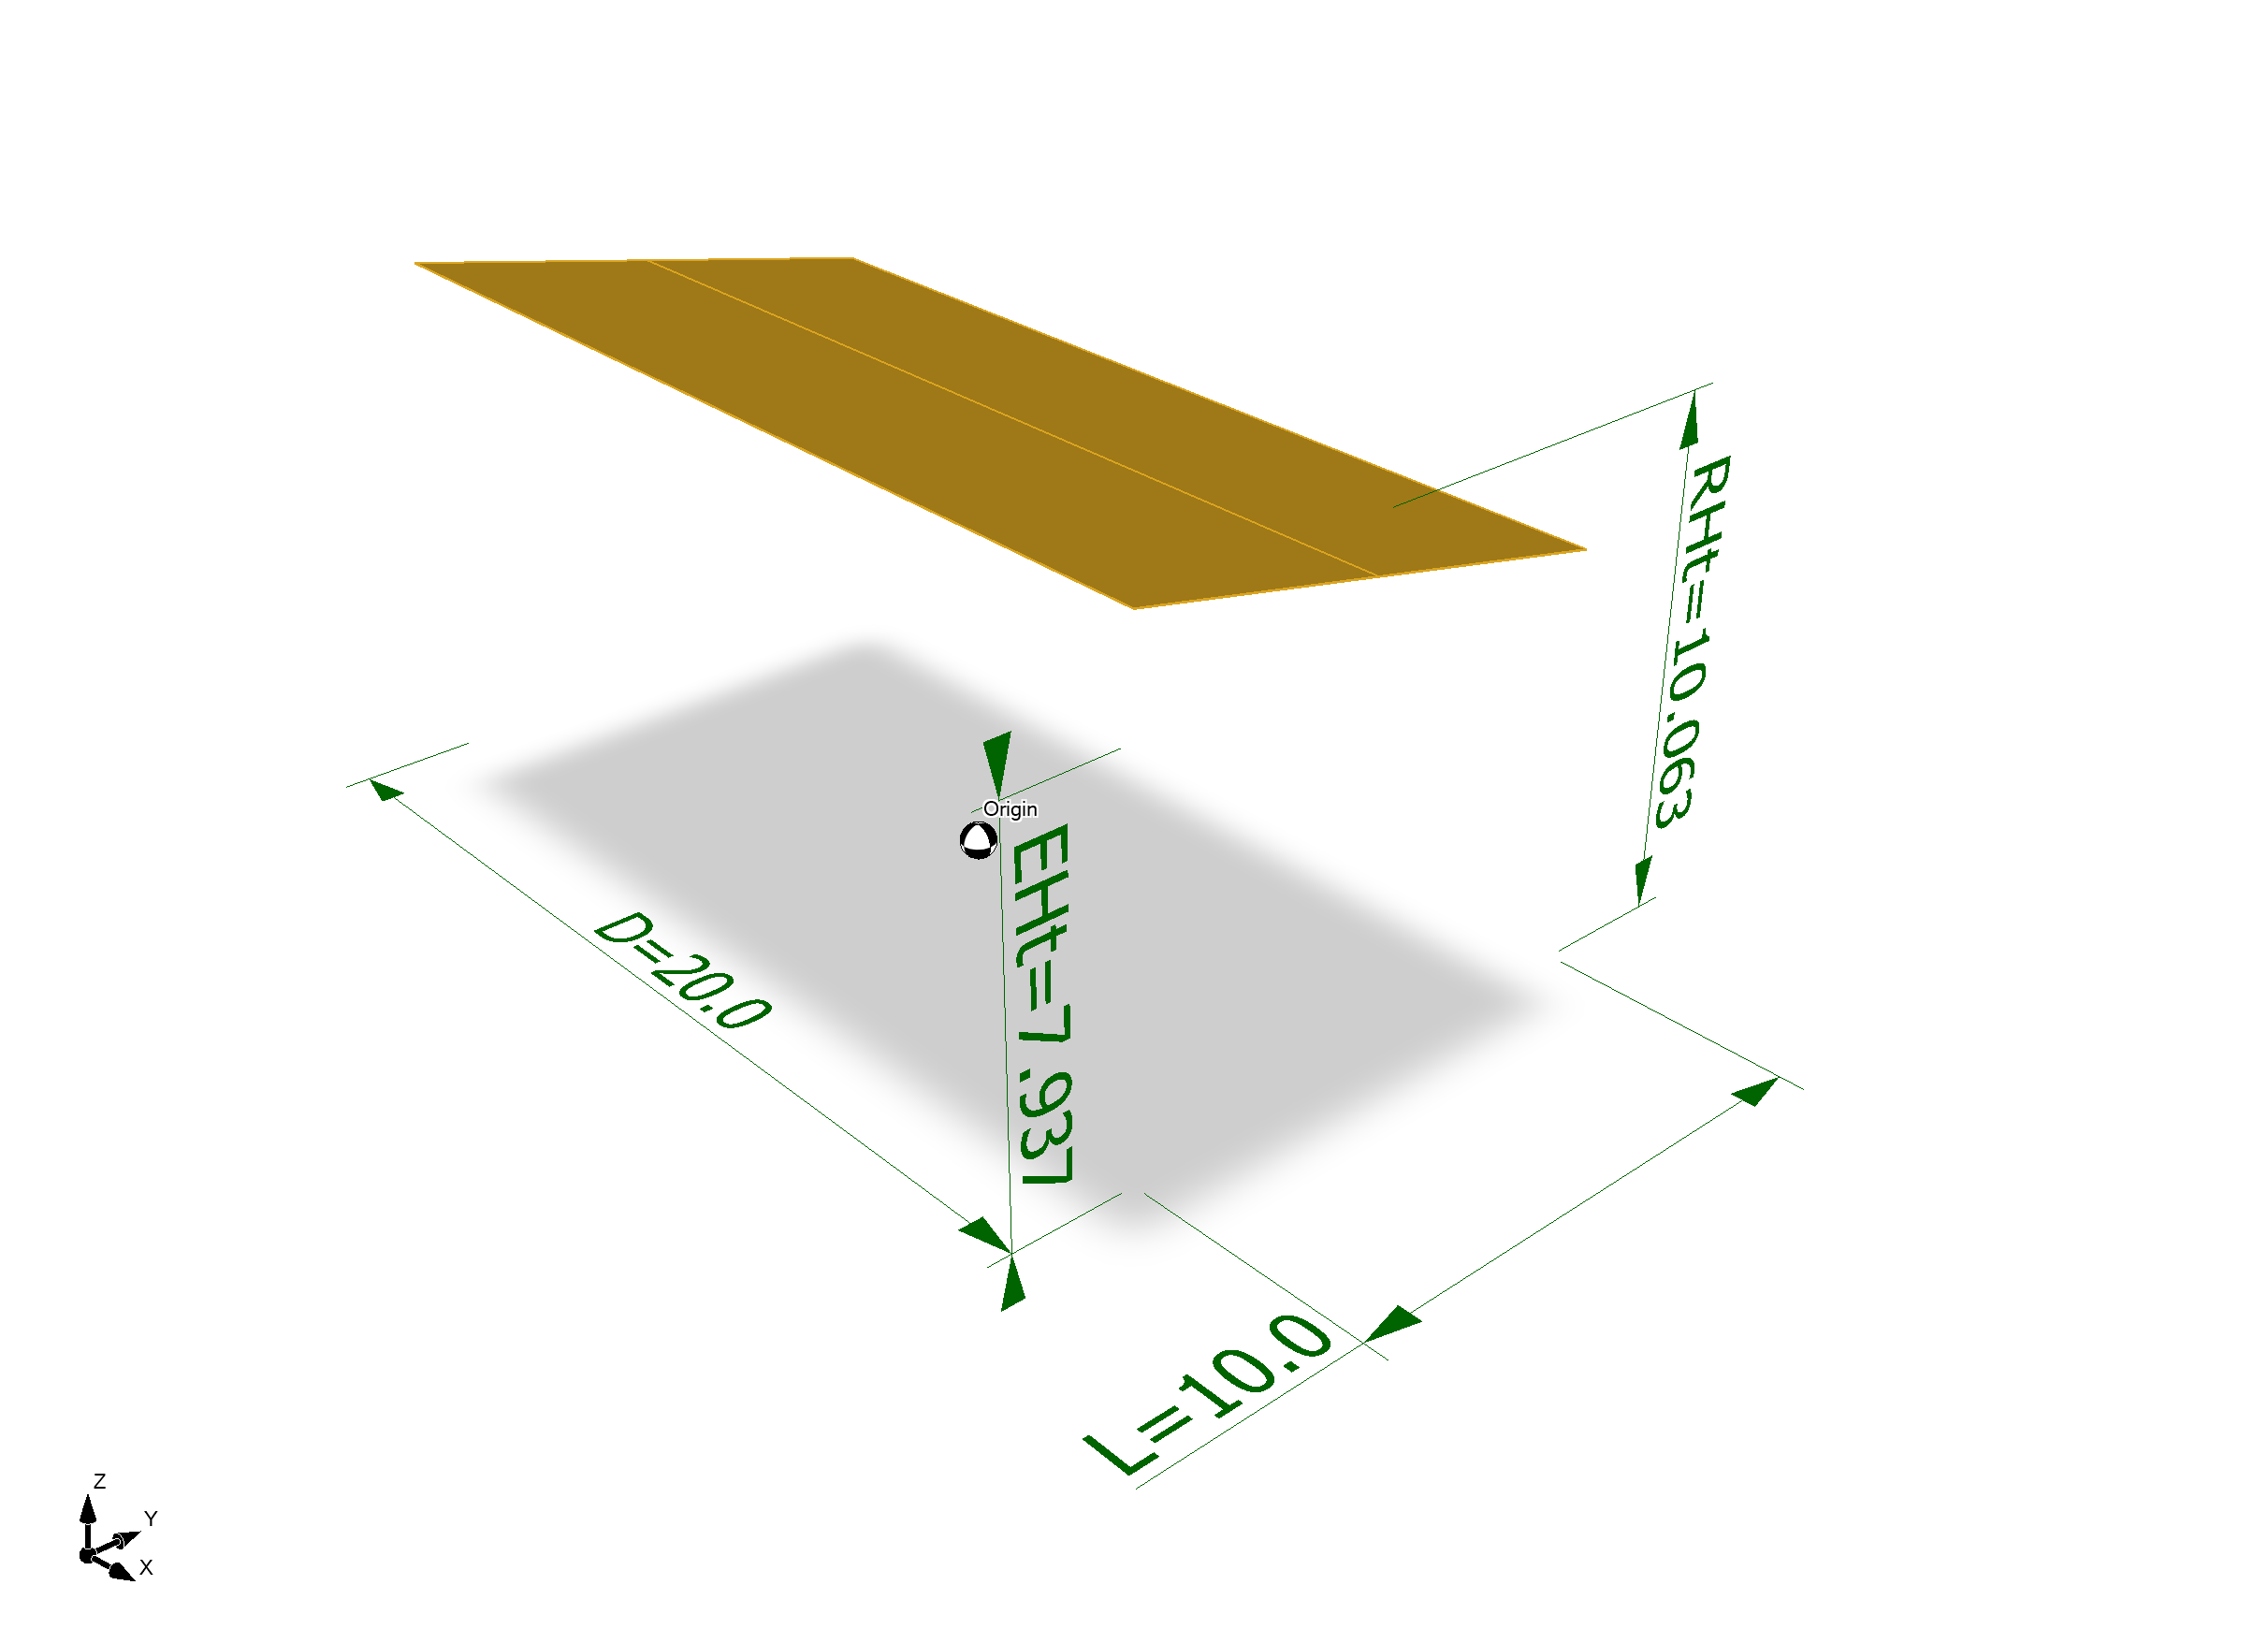
\includegraphics[scale=0.150000]{C:/git/rivtlocal-solar-canopy/rv01-loads/fig1.png}}

\vspace{.05in}

\textbf{Figure 1: Wind load 1}  \hfill 02 - F01

  \vspace{.05in}

\nopagebreak

\noindent\makebox[\linewidth][c]{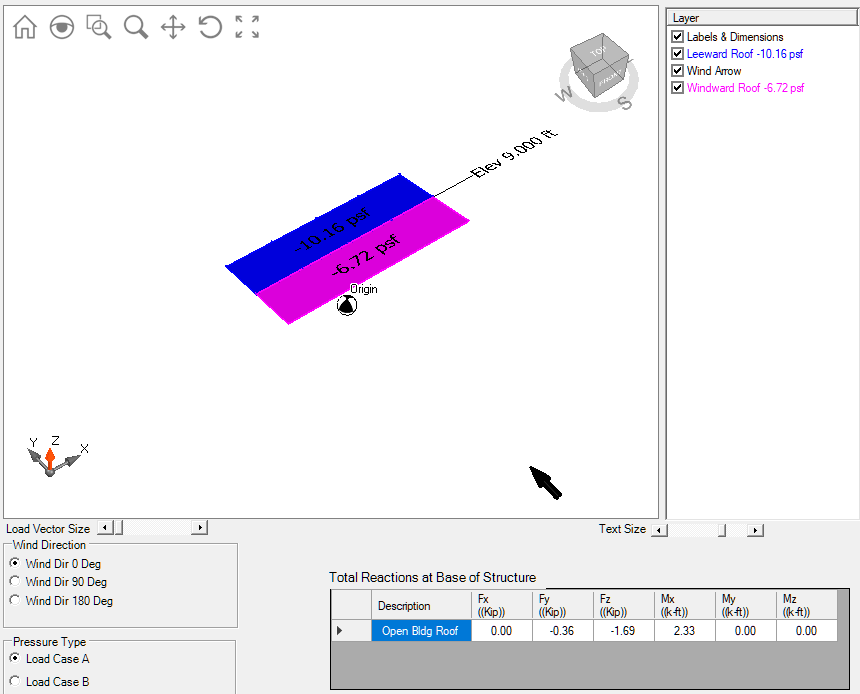
\includegraphics[scale=0.400000]{C:/git/rivtlocal-solar-canopy/rv01-loads/fig2.png}}

\vspace{.05in}

\textbf{Figure 2: Wind load 2}  \hfill 02 - F02

  \vspace{.05in}

\nopagebreak

\vspace{.05in}

\textbf{Table 01: Standards}  \hfill 02 - T01

  \vspace{.05in}

\nopagebreak

\setlength{\DUtablewidth}{\linewidth}%
\begin{longtable*}{|p{0.610\DUtablewidth}|p{0.133\DUtablewidth}|p{0.086\DUtablewidth}|}
\hline
\textbf{%
Category
} & \textbf{%
Standard
} & \textbf{%
Year
} \\
\hline
\endfirsthead
\hline
\textbf{%
Category
} & \textbf{%
Standard
} & \textbf{%
Year
} \\
\hline
\endhead
\multicolumn{3}{p{0.83\DUtablewidth}}{\raggedleft\ldots continued on next page}\\
\endfoot
\endlastfoot

Loading
 & 
ASCE-7
 & 
2016
 \\
\hline

Concrete
 & 
ACI-318
 & 
2014
 \\
\hline

Wood-National Design Specifications
 & 
AWC-NDS
 & 
2018
 \\
\hline

Wood-Special Design Provisions for Wind and Seismic
 & 
AWC-SDPWS
 & 
2015
 \\
\hline

Wood Frame Construction Manual
 & 
AWC-WFCM
 & 
2018
 \\
\hline
\end{longtable*}

\vspace{.05in}

\textbf{Table 02: Load Types}  \hfill 02 - T02

  \vspace{.05in}

\nopagebreak

\setlength{\DUtablewidth}{\linewidth}%
\begin{longtable*}{|p{0.075\DUtablewidth}|p{0.424\DUtablewidth}|p{0.424\DUtablewidth}|}
\hline
\textbf{%
Sym
} & \textbf{%
Load Effect
} & \textbf{%
Notes
} \\
\hline
\endfirsthead
\hline
\textbf{%
Sym
} & \textbf{%
Load Effect
} & \textbf{%
Notes
} \\
\hline
\endhead
\multicolumn{3}{p{0.92\DUtablewidth}}{\raggedleft\ldots continued on next page}\\
\endfoot
\endlastfoot

D
 & 
Dead load
 & 
See IBC 1606 and Chapter 3 of this
publication
 \\
\hline

E
 & 
Combined effect of horizontal and
vertical earthquake-induced forces
as defined in ASCE/SEI 12.4.2
 & 
See IBC 1613, ASCE/SEI 12.4.2 and
Chapter 6 of this publication
 \\
\hline

Em
 & 
Maximum seismic load effect of
horizontal and vertical forces as
set forth in ASCE/SEI 12.4.3
 & 
See IBC 1613, ASCE/SEI 12.4.3 and
Chapter 6 of this publication
 \\
\hline

H
 & 
Load due to lateral earth
pressures, ground water pressure or
pressure of bulk materials
 & 
See IBC 1610 for soil lateral loads
 \\
\hline

L
 & 
Live load, except roof live load,
including any permitted live load
reduction
 & 
See IBC 1607 and Chapter 3 of this
publication
 \\
\hline

Li
 & 
Roof live load including any
permitted live load reduction
 & 
See IBC 1607 and Chapter 3 of this
publication
 \\
\hline

R
 & 
Rain load
 & 
See IBC 1611 and Chapter 3 of this
publication
 \\
\hline

W
 & 
Load due to wind pressure
 & 
See IBC 1609 and Chapter 5 of this
publication
 \\
\hline
\end{longtable*}

\vspace{.05in}

\textbf{Table 03: Load Combinations}  \hfill 02 - T03

  \vspace{.05in}

\nopagebreak

\setlength{\DUtablewidth}{\linewidth}%
\begin{longtable*}{|p{0.249\DUtablewidth}|p{0.633\DUtablewidth}|}
\hline
\textbf{%
CBC 2019 reference
} & \textbf{%
Equation
} \\
\hline
\endfirsthead
\hline
\textbf{%
CBC 2019 reference
} & \textbf{%
Equation
} \\
\hline
\endhead
\multicolumn{2}{p{0.88\DUtablewidth}}{\raggedleft\ldots continued on next page}\\
\endfoot
\endlastfoot

Equation 16-1
 & 
1.4(D +F)
 \\
\hline

Equation 16-2
 & 
1.2(D + F) + l.6(L + H) + 0.5(L
 \\
\hline

Equation 16-3
 & 
1.2(D + F) + l.6(Lr or S or R) + l.6H + (f1L or 0.5W)
 \\
\hline

Equation 16-4
 & 
1.2(D + F) + 1.0W + f1L +1.6H + 0.5(Lr or S or R)
 \\
\hline

Equation 16-5
 & 
1.2(D + F) + 1.0E + f1L + l.6H + f2S
 \\
\hline

Equation 16-6
 & 
0.9D+ l.0W+ l.6H
 \\
\hline

Equation 16-7
 & 
0.9(D + F) + 1.0E+ l.6H
 \\
\hline
\end{longtable*}

\vspace{.2in}    \begin{tcolorbox}    \textbf{ Gravity Loads and Seismic Mass} \hfill\textbf{SECTION [0101] - 3 }   \end{tcolorbox}
  \newline   \vspace{.05in}

\vspace{.05in}

\textbf{Table 04: Roof unit dead loads}  \hfill 03 - T04

  \vspace{.05in}

\nopagebreak

\setlength{\DUtablewidth}{\linewidth}%
\begin{longtable*}{|p{0.133\DUtablewidth}|p{0.098\DUtablewidth}|p{0.121\DUtablewidth}|p{0.400\DUtablewidth}|}
\hline
\textbf{%
variable
} & \textbf{%
value
} & \textbf{%
{[}value{]}
} & \textbf{%
description
} \\
\hline
\endfirsthead
\hline
\textbf{%
variable
} & \textbf{%
value
} & \textbf{%
{[}value{]}
} & \textbf{%
description
} \\
\hline
\endhead
\multicolumn{4}{p{0.75\DUtablewidth}}{\raggedleft\ldots continued on next page}\\
\endfoot
\endlastfoot

ld1
 & 
2.0 psf
 & 
0.10 KPa
 & 
Urethane foam (4 inch thick)
 \\
\hline

ld2
 & 
1.0 psf
 & 
0.05 KPa
 & 
Three-ply roofing
 \\
\hline

ld3
 & 
5.0 psf
 & 
0.24 KPa
 & 
Doug Fir decking 2-in.
 \\
\hline

ld4
 & 
1.0 psf
 & 
0.05 KPa
 & 
Doug Fir beams 4x12 at 12 ft o.c.
 \\
\hline

\_ \_
 & 
\_ \_
 & 
\_ \_
 & 
Total
 \\
\hline

roofdl1
 & 
9.0 psf
 & 
0.43 KPa
 & 
Total roof unit load
 \\
\hline
\end{longtable*}

\vspace{.05in}

\textbf{Table 05: Floor unit dead loads}  \hfill 03 - T05

  \vspace{.05in}

\nopagebreak

\setlength{\DUtablewidth}{\linewidth}%
\begin{longtable*}{|p{0.133\DUtablewidth}|p{0.110\DUtablewidth}|p{0.121\DUtablewidth}|p{0.319\DUtablewidth}|}
\hline
\textbf{%
variable
} & \textbf{%
value
} & \textbf{%
{[}value{]}
} & \textbf{%
description
} \\
\hline
\endfirsthead
\hline
\textbf{%
variable
} & \textbf{%
value
} & \textbf{%
{[}value{]}
} & \textbf{%
description
} \\
\hline
\endhead
\multicolumn{4}{p{0.68\DUtablewidth}}{\raggedleft\ldots continued on next page}\\
\endfoot
\endlastfoot

ld1
 & 
3.0 psf
 & 
0.14 KPa
 & 
3/4 in. hardwood flooring
 \\
\hline

ld2
 & 
2.0 psf
 & 
0.10 KPa
 & 
1/2 in. plywood subfloor
 \\
\hline

ld3
 & 
4.0 psf
 & 
0.19 KPa
 & 
2x10 joists at 16 in. o.c.
 \\
\hline

ld4
 & 
1.5 psf
 & 
0.07 KPa
 & 
fixtures
 \\
\hline

\_ \_
 & 
\_ \_
 & 
\_ \_
 & 
Total
 \\
\hline

floordl1
 & 
10.5 psf
 & 
0.50 KPa
 & 
Total floor unit load
 \\
\hline
\end{longtable*}

\vspace{.05in}

\textbf{Table 06: Interior wall unit dead loads}  \hfill 03 - T06

  \vspace{.05in}

\nopagebreak

\setlength{\DUtablewidth}{\linewidth}%
\begin{longtable*}{|p{0.133\DUtablewidth}|p{0.098\DUtablewidth}|p{0.121\DUtablewidth}|p{0.354\DUtablewidth}|}
\hline
\textbf{%
variable
} & \textbf{%
value
} & \textbf{%
{[}value{]}
} & \textbf{%
description
} \\
\hline
\endfirsthead
\hline
\textbf{%
variable
} & \textbf{%
value
} & \textbf{%
{[}value{]}
} & \textbf{%
description
} \\
\hline
\endhead
\multicolumn{4}{p{0.71\DUtablewidth}}{\raggedleft\ldots continued on next page}\\
\endfoot
\endlastfoot

ld1
 & 
5.5 psf
 & 
0.26 KPa
 & 
5/8\textquotedbl{} sheet rock (2)
 \\
\hline

ld2
 & 
2 psf
 & 
0.10 KPa
 & 
2x4 studs at 16\textquotedbl{} o.c.
 \\
\hline

ld3
 & 
1.5 psf
 & 
0.07 KPa
 & 
fixtures
 \\
\hline

\_ \_
 & 
\_ \_
 & 
\_ \_
 & 
Total
 \\
\hline

intwalldl1
 & 
9 psf
 & 
0.43 KPa
 & 
Total interior wall unit load
 \\
\hline
\end{longtable*}

\vspace{.05in}

\textbf{Table 07: Exterior wall unit dead loads}  \hfill 03 - T07

  \vspace{.05in}

\nopagebreak

\setlength{\DUtablewidth}{\linewidth}%
\begin{longtable*}{|p{0.133\DUtablewidth}|p{0.098\DUtablewidth}|p{0.121\DUtablewidth}|p{0.354\DUtablewidth}|}
\hline
\textbf{%
variable
} & \textbf{%
value
} & \textbf{%
{[}value{]}
} & \textbf{%
description
} \\
\hline
\endfirsthead
\hline
\textbf{%
variable
} & \textbf{%
value
} & \textbf{%
{[}value{]}
} & \textbf{%
description
} \\
\hline
\endhead
\multicolumn{4}{p{0.71\DUtablewidth}}{\raggedleft\ldots continued on next page}\\
\endfoot
\endlastfoot

ld1
 & 
2.0 psf
 & 
0.10 KPa
 & 
1/2 in plywood sheathing
 \\
\hline

ld2
 & 
2.0 psf
 & 
0.10 KPa
 & 
2x4 studs at 16 in o.c.
 \\
\hline

ld3
 & 
3.0 psf
 & 
0.14 KPa
 & 
5/8 in sheet rock
 \\
\hline

ld4
 & 
1.5 psf
 & 
0.07 KPa
 & 
fixtures
 \\
\hline

\_ \_
 & 
\_ \_
 & 
\_ \_
 & 
Total
 \\
\hline

extwalldl1
 & 
8.5 psf
 & 
0.41 KPa
 & 
Total exterior wall unit load
 \\
\hline
\end{longtable*}

\vspace{.05in}

\textbf{Table 08: Areas}  \hfill 03 - T08

  \vspace{.05in}

\nopagebreak

\setlength{\DUtablewidth}{\linewidth}%
\begin{longtable*}{|p{0.133\DUtablewidth}|p{0.133\DUtablewidth}|p{0.121\DUtablewidth}|p{0.272\DUtablewidth}|}
\hline
\textbf{%
variable
} & \textbf{%
value
} & \textbf{%
{[}value{]}
} & \textbf{%
description
} \\
\hline
\endfirsthead
\hline
\textbf{%
variable
} & \textbf{%
value
} & \textbf{%
{[}value{]}
} & \textbf{%
description
} \\
\hline
\endhead
\multicolumn{4}{p{0.66\DUtablewidth}}{\raggedleft\ldots continued on next page}\\
\endfoot
\endlastfoot

arearf1
 & 
1700.00 sf
 & 
157.94 SM
 & 
roof area
 \\
\hline

areaflr1
 & 
1200.00 sf
 & 
111.48 SM
 & 
floor area
 \\
\hline

htwall1
 & 
9.00 ft
 & 
2.74 m
 & 
wall height
 \\
\hline

lenwall1
 & 
110.00 ft
 & 
33.53 m
 & 
interior wall length
 \\
\hline

lenwall2
 & 
155.00 ft
 & 
47.24 m
 & 
exterior wall length 2
 \\
\hline
\end{longtable*}

\textbf{Eq. 1: Roof weight}  \hfill 03 - E01

\begin{quote}
\begin{alltt}
rfwt₁ = arearf₁⋅roofdl₁
\end{alltt}
\end{quote}

\begin{quote}
\begin{alltt}
15.30 kip = 1700.00 sf⋅9.00 psf
\end{alltt}
\end{quote}

\textbf{Eq. 2: Floor weight}  \hfill 03 - E02

\begin{quote}
\begin{alltt}
flrwt₁ = areaflr₁⋅floordl₁
\end{alltt}
\end{quote}

\begin{quote}
\begin{alltt}
12.60 kip = 10.50 psf⋅1200.00 sf
\end{alltt}
\end{quote}

\textbf{Eq. 3: Partition weight}  \hfill 03 - E03

\begin{quote}
\begin{alltt}
partwt₁ = htwall₁⋅intwalldl₁⋅lenwall₁
\end{alltt}
\end{quote}

\begin{quote}
\begin{alltt}
8.91 kip = 110.00 ft⋅9.00 ft⋅9.00 psf
\end{alltt}
\end{quote}

\textbf{Eq. 4: Exterior wall weight}  \hfill 03 - E04

\begin{quote}
\begin{alltt}
exwallwt₁ = extwalldl₁⋅htwall₁⋅lenwall₂
\end{alltt}
\end{quote}

\begin{quote}
\begin{alltt}
11.86 kip = 155.00 ft⋅8.50 psf⋅9.00 ft
\end{alltt}
\end{quote}

\textbf{Eq. 5: Total building weight}  \hfill 03 - E05

\begin{quote}
\begin{alltt}
totwt₁ = exwallwt₁ + flrwt₁ + partwt₁ + rfwt₁
\end{alltt}
\end{quote}

\begin{quote}
\begin{alltt}
48.67 kip = 11857.50 lbs + 12600.00 lbs + 15300.00 lbs + 8910.00 lbs
\end{alltt}
\end{quote}

\vspace{.05in}

\textbf{Table 09: Weights}  \hfill 03 - T09

  \vspace{.05in}

\nopagebreak

\setlength{\DUtablewidth}{\linewidth}%
\begin{longtable*}{|p{0.133\DUtablewidth}|p{0.121\DUtablewidth}|p{0.121\DUtablewidth}|p{0.331\DUtablewidth}|}
\hline
\textbf{%
variable
} & \textbf{%
value
} & \textbf{%
{[}value{]}
} & \textbf{%
description {[}eq. number{]}
} \\
\hline
\endfirsthead
\hline
\textbf{%
variable
} & \textbf{%
value
} & \textbf{%
{[}value{]}
} & \textbf{%
description {[}eq. number{]}
} \\
\hline
\endhead
\multicolumn{4}{p{0.71\DUtablewidth}}{\raggedleft\ldots continued on next page}\\
\endfoot
\endlastfoot

rfwt1
 & 
15.30 kip
 & 
68.06 KN
 & 
Roof weight  {[}01{]}
 \\
\hline

flrwt1
 & 
12.60 kip
 & 
56.05 KN
 & 
Floor weight  {[}02{]}
 \\
\hline

partwt1
 & 
8.91 kip
 & 
39.63 KN
 & 
Partition weight  {[}03{]}
 \\
\hline

exwallwt1
 & 
11.86 kip
 & 
52.74 KN
 & 
Exterior wall weight  {[}04{]}
 \\
\hline

totwt1
 & 
48.67 kip
 & 
216.48 KN
 & 
Total building weight  {[}05{]}
 \\
\hline
\end{longtable*}

\vspace{.2in}    \begin{tcolorbox}    \textbf{ Material Densities and Seismic Models} \hfill\textbf{SECTION [0101] - 4 }   \end{tcolorbox}
  \newline   \vspace{.05in}

\textbf{Eq. 6: Effective model floor load}  \hfill 04 - E06

\begin{quote}
\begin{alltt}
          flrwt₁ + partwt₁
eflrdl₁ = ────────────────
              areaflr₁
\end{alltt}
\end{quote}

\begin{quote}
\begin{alltt}
            12600.00 lbs + 8910.00 lbs
17.93 psf = ──────────────────────────
                    1200.00 sf
\end{alltt}
\end{quote}

\textbf{Eq. 7: Effective model floor density}  \hfill 04 - E07

\begin{quote}
\begin{alltt}
            eflrdl₁
eflrdens₁ = ───────
             0.5⋅IN
\end{alltt}
\end{quote}

\begin{quote}
\begin{alltt}
           17.93 lbs/sf
0.25 pci = ────────────
              0.5⋅in
\end{alltt}
\end{quote}

\textbf{Eq. 8: Effective model roof density}  \hfill 04 - E08

\begin{quote}
\begin{alltt}
           roofdl₁
erfdens₁ = ───────
            1.5⋅IN
\end{alltt}
\end{quote}

\begin{quote}
\begin{alltt}
           9.00 psf
0.04 pci = ────────
            1.5⋅in
\end{alltt}
\end{quote}

\textbf{Eq. 9: Effective model wall density}  \hfill 04 - E09

\begin{quote}
\begin{alltt}
             extwalldl₁
ewalldens₁ = ──────────
               0.5⋅IN
\end{alltt}
\end{quote}

\begin{quote}
\begin{alltt}
           8.50 psf
0.12 pci = ────────
            0.5⋅in
\end{alltt}
\end{quote}

\vspace{.05in}

\textbf{Table 10: Model loads}  \hfill 04 - T10

  \vspace{.05in}

\nopagebreak

\setlength{\DUtablewidth}{\linewidth}%
\begin{longtable*}{|p{0.133\DUtablewidth}|p{0.121\DUtablewidth}|p{0.133\DUtablewidth}|p{0.424\DUtablewidth}|}
\hline
\textbf{%
variable
} & \textbf{%
value
} & \textbf{%
{[}value{]}
} & \textbf{%
description {[}eq. number{]}
} \\
\hline
\endfirsthead
\hline
\textbf{%
variable
} & \textbf{%
value
} & \textbf{%
{[}value{]}
} & \textbf{%
description {[}eq. number{]}
} \\
\hline
\endhead
\multicolumn{4}{p{0.81\DUtablewidth}}{\raggedleft\ldots continued on next page}\\
\endfoot
\endlastfoot

eflrdl1
 & 
17.93 psf
 & 
0.86 KPa
 & 
Effective model floor load   {[}06{]}
 \\
\hline

eflrdens1
 & 
0.25 pci
 & 
67.58 KNcM
 & 
Effective model floor density  {[}07{]}
 \\
\hline

erfdens1
 & 
0.04 pci
 & 
11.31 KNcM
 & 
Effective model roof density  {[}08{]}
 \\
\hline

ewalldens1
 & 
0.12 pci
 & 
32.05 KNcM
 & 
Effective model wall density  {[}09{]}
 \\
\hline
\end{longtable*}

\vspace{.2in}    \begin{tcolorbox}    \textbf{ Abbreviations and References} \hfill\textbf{SECTION [0101] - 5 }   \end{tcolorbox}
  \newline   \vspace{.05in}

\begin{center} \textbf{References } \end{center}

\begin{quote}
\begin{alltt}
ACI
American Concrete Institute
38800 Country Club Drive
Farmington Hills, MI 48331
318—14

AISC
American Institute of Steel
130 East Randolph Street, Suite 2000
Chicago, IL 60601-6219
ANSI/AISC 341—16
Seismic Provisions for Structural Steel Buildings

AISI
American Iron and Steel Institute
25 Massachusetts Avenue, NW Suite 800
Washington, DC 20001
AISI S100—16
North American Specification for the Design of Cold-formed
Steel Structural Members, 2016

ASCE/SEI
American Society of Civil Engineers
Structural Engineering Institute
1801 Alexander Bell Drive
Reston, VA 20191-4400
7—16 Minimum Design Loads and Associated Criteria for
Buildings and Other Structures with Supplement No. 1

AWC
American Wood Council
222 Catoctin Circle SE, Suite 201
Leesburg, VA 20175
ANSI/AWC NDS—2018
National Design Specification (NDS) for
Wood Construction—with 2018 NDS Supplement
ANSI/AWC SDPWS—2015
Special Design Provisions for Wind and Seismic

CBC
International Code Council
500 New Jersey Avenue, NW
6th Floor, Washington, DC 20001
California Building Standards Commission
2525 Natomas Park Dr # 130, Sacramento, CA 95833
California Building Code
Part 2 of Title 24, 2019 Edition

CRC
International Code Council
500 New Jersey Avenue, NW
6th Floor, Washington, DC 20001
California Building Standards Commission
2525 Natomas Park Dr # 130, Sacramento, CA 95833
California Residential Code
Part 2.5 of Title 24, 2019 Edition
\end{alltt}
\end{quote}

\begin{center} \textbf{Drawings } \end{center}

\begin{quote}
\begin{alltt}
55 LORING - RESIDENCE REMODEL AND SEISMIC STRENGTHENING

PR.01: COVER AND INDEX
PR.02: PROJECT SCOPE
PR.03: GENERAL NOTES, CONTRACTORS
PR.04: SITE PLAN
PR.05: PLANS
PR.06: ELEVATIONS
PR.07: KITCHEN AND BATH REMODEL
PR.08: MASTER BATH, CLOSET, LAUNDRY
PR.09: RESIDENCE STRENGTHENING
PR.10: CARPORT STRENGTHENING
PR.11: SITE IMPROVEMENTS
\end{alltt}
\end{quote}

\begin{center} \textbf{Abbreviations - Terms } \end{center}

\setlength{\parindent}{0.2in}
\vspace{-0.3in}
\begin{tabbing}
\hspace*{4cm} \= \kill
    \indent\textbf{}         \>  {}\\
    \indent\textbf{ASD}      \>  {Allowable Stress Design}\\
    \indent\textbf{ACI}      \>  {American Concrete Institute}\\
    \indent\textbf{AISC}     \>  {American Institute of Steel Construction}\\
    \indent\textbf{AISI}     \>  {American Iron and Steel Institute}\\
    \indent\textbf{ASTM}     \>  {American Society for Testing and Materials}\\
    \indent\textbf{AWS}      \>  {American Welding Society}\\
    \indent\textbf{AB}       \>  {Anchor Bolt}\\
    \indent\textbf{BDRY}     \>  {Boundry}\\
    \indent\textbf{CBC}      \>  {Califiornia Building Code}\\
    \indent\textbf{CRC}      \>  {Califiornia Residential Code}\\
    \indent\textbf{CIP}      \>  {Cast-In-Place}\\
    \indent\textbf{CLR}      \>  {Clear}\\
    \indent\textbf{CONC}     \>  {Concrete}\\
    \indent\textbf{CMU}      \>  {Concrete Masonry Unit}\\
    \indent\textbf{CRSI}     \>  {Concrete Reinforcing Steel Institute}\\
    \indent\textbf{CONST JT} \>  {Construction Joint}\\
    \indent\textbf{CONT}     \>  {Continuous}\\
    \indent\textbf{CJ}       \>  {Control Joint}\\
    \indent\textbf{D-C}      \>  {Demand-Capacity (ratio)}\\
    \indent\textbf{DIA}      \>  {Diameter}\\
    \indent\textbf{DIM}      \>  {Dimension}\\
    \indent\textbf{EA}       \>  {Each}\\
    \indent\textbf{EF}       \>  {Each Face}\\
    \indent\textbf{EJ}       \>  {Expansion Joint}\\
    \indent\textbf{ES}       \>  {Each Side}\\
    \indent\textbf{EW}       \>  {Each Way}\\
    \indent\textbf{EXP Bolt} \>  {Expansion Bolt}\\
    \indent\textbf{EXP JT}   \>  {Expansion Joint}\\
    \indent\textbf{FTG}      \>  {Footing}\\
    \indent\textbf{FND}      \>  {Foundation}\\
    \indent\textbf{GALV}     \>  {Galvanized}\\
    \indent\textbf{GA}       \>  {Gauge}\\
    \indent\textbf{GR}       \>  {Grade}\\
    \indent\textbf{HT}       \>  {Height}\\
    \indent\textbf{IN}       \>  {Inch}\\
    \indent\textbf{ID}       \>  {Inside Diameter}\\
    \indent\textbf{ICBO}     \>  {International Conference of Building Officials}\\
    \indent\textbf{K}        \>  {Kip (1000 Pounds)}\\
    \indent\textbf{LWC}      \>  {Light Weight Concrete}\\
    \indent\textbf{LRFD}     \>  {Load and Resistance Factor Design}\\
    \indent\textbf{NWC}      \>  {Normal Weight Concrete}\\
    \indent\textbf{NIC}      \>  {Not in Contract}\\
    \indent\textbf{OC}       \>  {On Center}\\
    \indent\textbf{OD}       \>  {Outside Diameter}\\
    \indent\textbf{OPNG}     \>  {Opening}\\
    \indent\textbf{PVC}      \>  {Polyvinyl Chloride}\\
    \indent\textbf{PSF}      \>  {Pounds per Square Foot}\\
    \indent\textbf{PSI}      \>  {Pounds per Square Inch}\\
    \indent\textbf{R}        \>  {Radius}\\
    \indent\textbf{REINF}    \>  {Reinforced}\\
    \indent\textbf{SIM}      \>  {Similar}\\
    \indent\textbf{SOG}      \>  {Slab on Grade}\\
    \indent\textbf{SL}       \>  {Splice Length}\\
    \indent\textbf{SQ}       \>  {Square}\\
    \indent\textbf{STD}      \>  {Standard}\\
    \indent\textbf{SDI}      \>  {Steel Deck Institute}\\
    \indent\textbf{SF}       \>  {Step Footing or Square Foot}\\
    \indent\textbf{SYM}      \>  {Symmetrical}\\
    \indent\textbf{THK}      \>  {Thick or Thickness}\\
    \indent\textbf{T \& B}   \>  {Top and Bottom}\\
    \indent\textbf{T \& G}   \>  {Tongue and Groove}\\
    \indent\textbf{TOC}      \>  {Top of Concrete}\\
    \indent\textbf{TOF}      \>  {Top of Foundation}\\
    \indent\textbf{TOS}      \>  {Top of Steel}\\
    \indent\textbf{TOW}      \>  {Top of Wall}\\
    \indent\textbf{TYP}      \>  {Typical}\\
    \indent\textbf{UNO}      \>  {Unless Noted Otherwise}\\
    \indent\textbf{WWF}      \>  {Welded Wire Fabric}\\
    \indent\textbf{W/}       \>  {With}\\
    \indent\textbf{WP}       \>  {Working Point}\\
\end{tabbing}

\begin{center} \textbf{Abbreviations - Math } \end{center}

\vspace{-.4in}
\begingroup
\allowdisplaybreaks
\begin{align*}
    \bm{D}       & = \textrm{dead load}                               \\
    \bm{L}       & = \textrm{live load}                               \\
    \bm{D_m}     & = \textrm{module dead load}                        \\
    \bm{E}       & = \textrm{earthquake load}                         \\
    \bm{F_a}     & = \textrm{acceleration site coefficient}           \\
    \bm{F_v}     & = \textrm{velocity site coefficient}               \\
    \bm{F_N}     & = \textrm{normal wind force}                       \\
    \bm{GC_M_s}  & = \textrm{net moment static coefficient}           \\
    \bm{GC_M_d}  & = \textrm{net moment dynamic coefficient}          \\
    \bm{GC_M}    & = \textrm{net moment coefficient}                  \\
    \bm{GC_P}    & = \textrm{net pressure coefficient}                \\
    \bm{GC_P_s}  & = \textrm{net static pressure coefficient}         \\
    \bm{GC_P_d}  & = \textrm{net dynamic pressure coefficient}        \\
    \bm{k_1}     & = \textrm{hazard coefficient}                      \\
    \bm{k_2}     & = \textrm{terrain and structure coefficient}       \\
    \bm{k_3}     & = \textrm{topography coefficient}                  \\
    \bm{Kzt}     & = \textrm{topographic Factor}                      \\
    \bm{K_z}     & = \textrm{velocity pressure exposure coefficient}  \\
    \bm{MRI}     & = \textrm{mean return interval}                    \\
    \bm{p_d}     & = \textrm{net design wind pressure on module - Pa} \\
    \bm{SDOF}    & = \textrm{single degree of freedom}                \\
    \bm{S_s}     & = \textrm{short period mapped acceleration}        \\
    \bm{S_D_S}   & = \textrm{site design response acceleration}       \\
    \bm{S_1}     & = \textrm{1 second period mapped acceleration}     \\
    \bm{S_M_S}   & = \textrm{short period parameter}                  \\
    \bm{S_M_1}   & = \textrm{1 second period parameter}               \\
    \bm{T}       & = \textrm{fundamental period of structure}         \\
    \bm{M_t_o_r} & = \textrm{wind moment about panel center }         \\
    \bm{T_0}     & = \textrm{short period spectral cap }              \\
    \bm{T_S}     & = \textrm{long period spectral cap}                \\
    \bm{V_b}     & = \textrm{basic wind speed}                        \\
    \bm{V_B}     & = \textrm{seismic design base shear}               \\
    \bm{W}       & = \textrm{wind load}                               \\
    \bm{W}       & = \textrm{seismic weight of structure }            \\
\end{align*}
\endgroup

\end{document}
